\chapter{Implementation}\label{ch:implementation}
To fulfill the assumptions of this work, the authors prepared a whole system that is able to collect and verify the mouse dynamics data.
The high-level flow of the system is presented in Fig.~\ref{fig:overall_system_structure} and provides the basis for further considerations.
\begin{figure}[!hbt]
    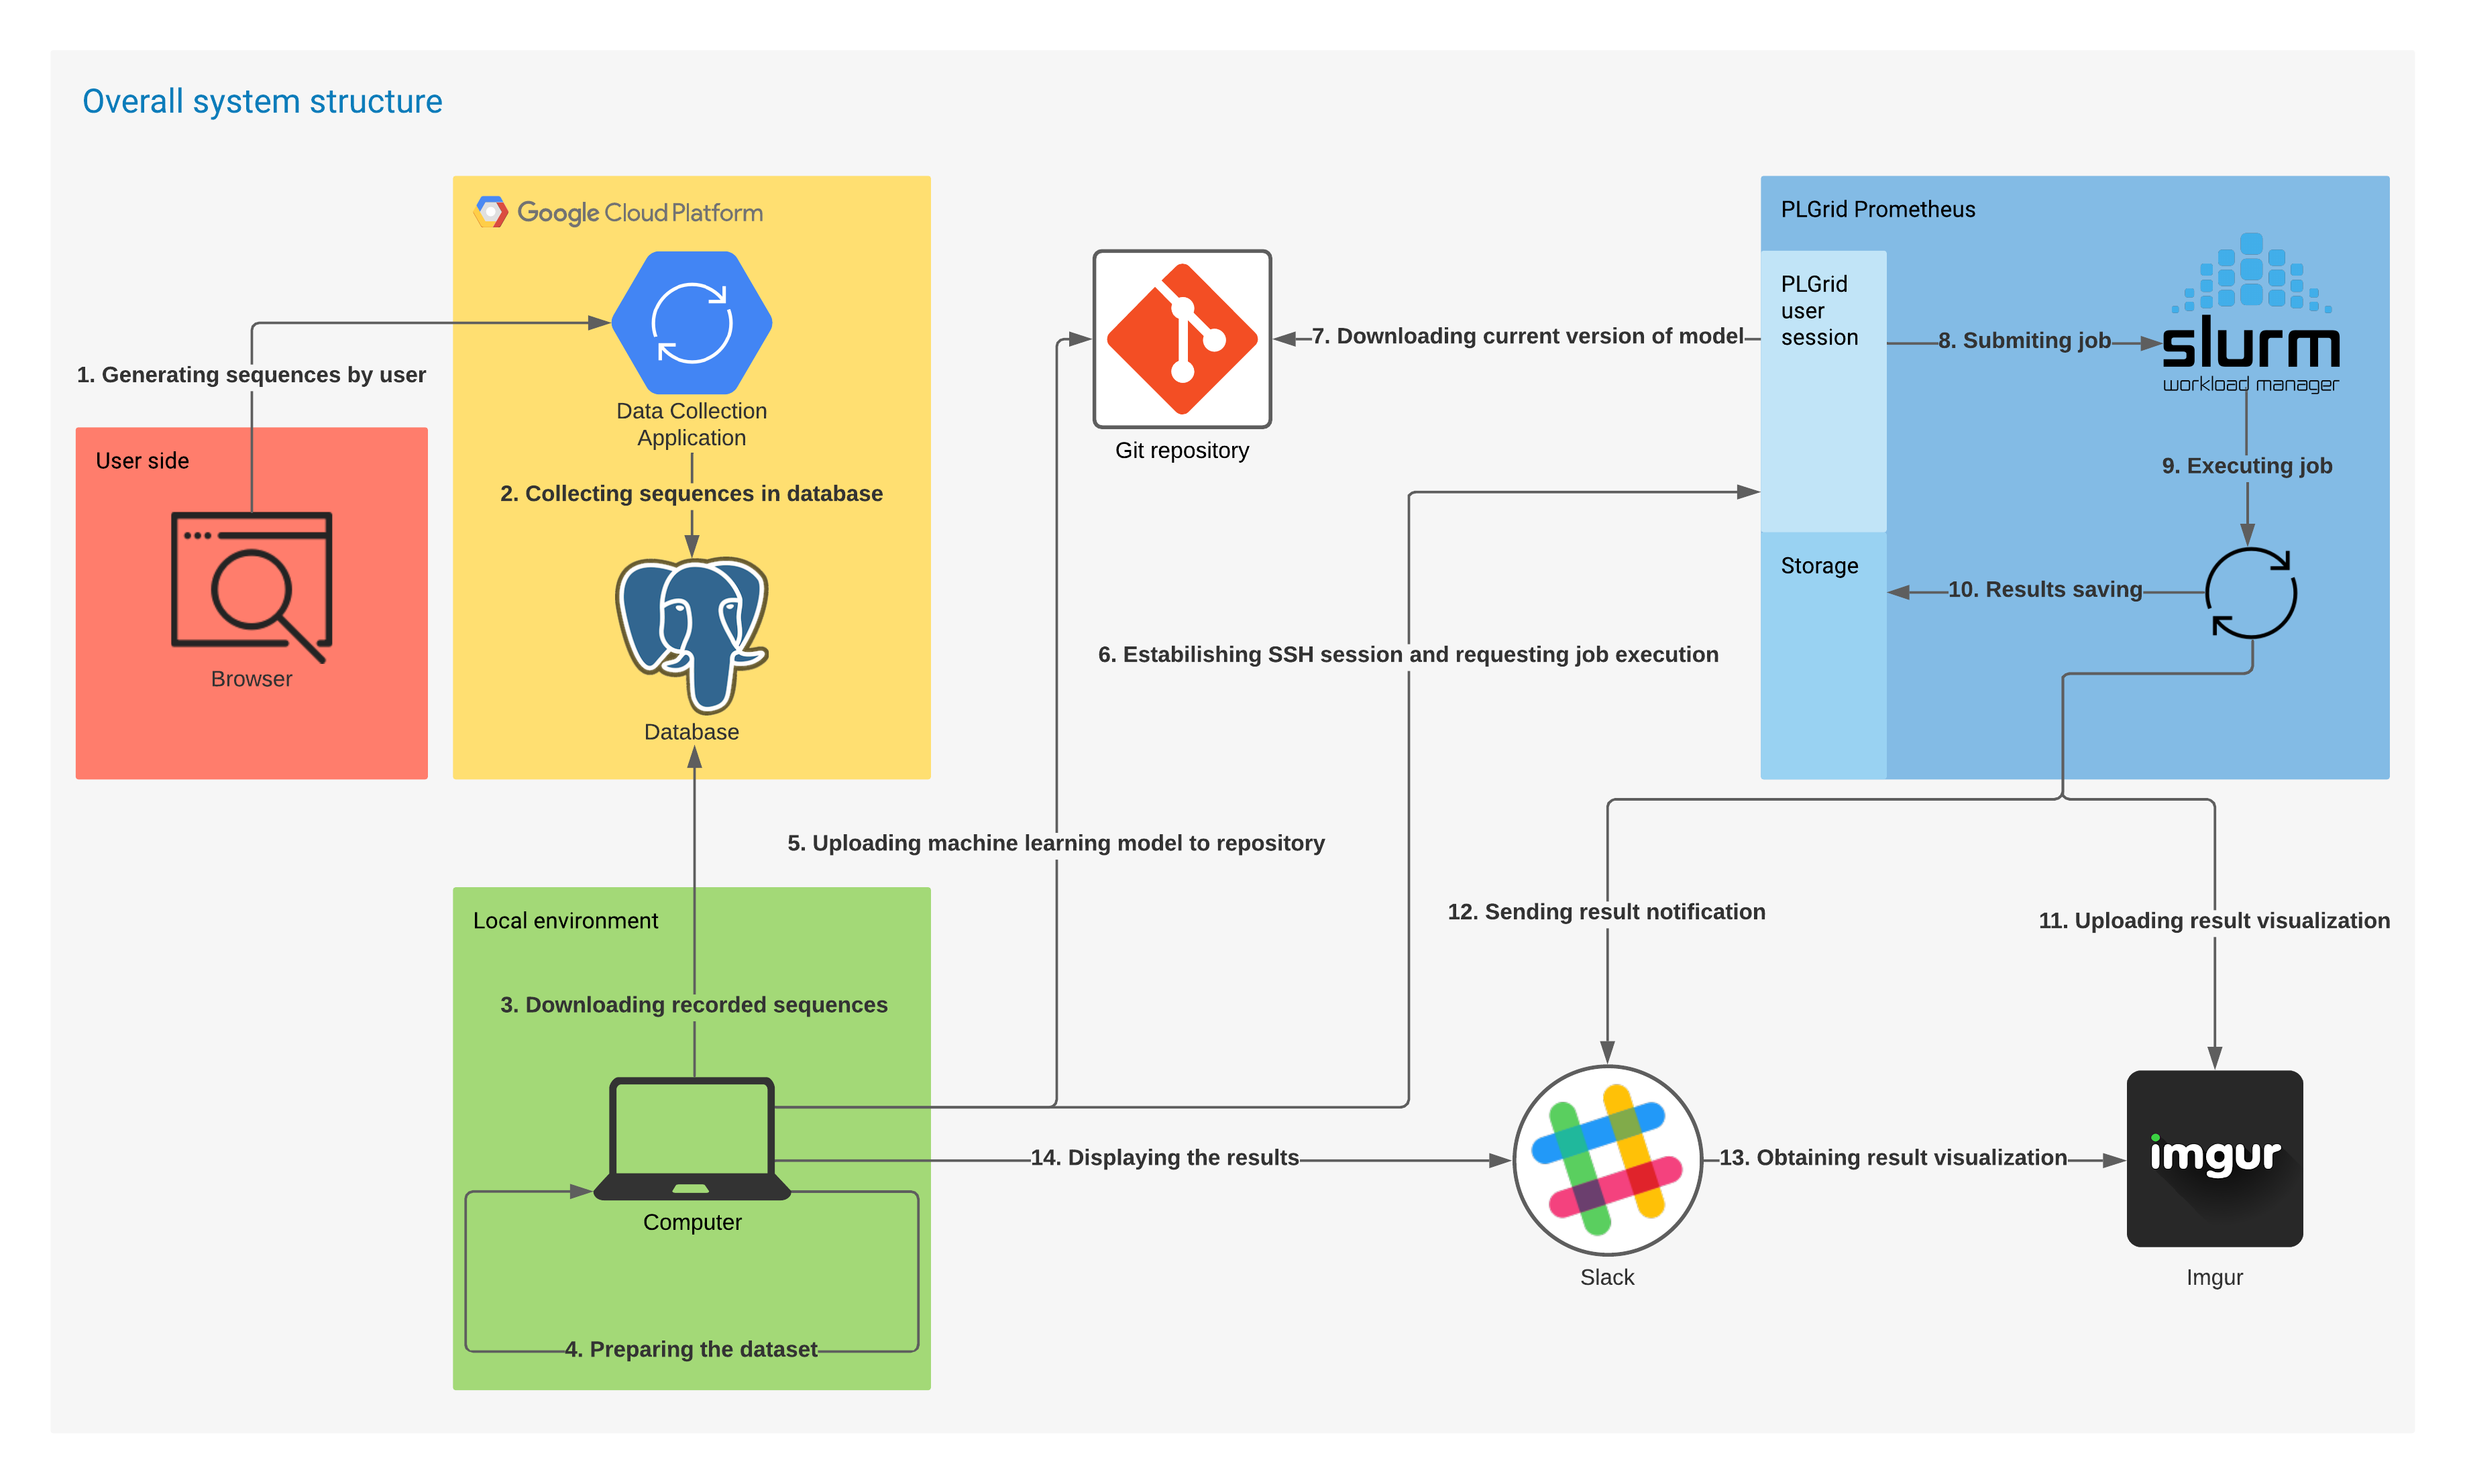
\includegraphics[width=\linewidth]{resources/overall_system_structure}
    \captionof{figure}{Overall system structure diagram}
    \label{fig:overall_system_structure}
\end{figure}

The entry point for the system is the user's browser that allows the human user as well as a human impersonating bot for access to the prepared website which is hosted on the Internet.
The \mbox{Data Collection}\upperref{itm:data-collection} module which is persisted and operates within a cloud acts as a mouse dynamics data collector, which means that every single mouse event generated by the user on the website is intercepted, transformed and stored in the underlying database (Fig.~\ref{fig:overall_system_structure}, pt. 1 and pt. 2).
The administrator of presented system is able to retrieve the data from the database in any time (pt. 3).
The downloaded data can be further processed (pt. 4) to the dataset which will be used in machine learning stage.
The administrator of the system should prepare a machine learning model and upload it to the Git repository (pt. 5) which will be then obtained by computing cluster to perform computation using the model from the observed branch.
Such an approach allows to work on the solution simultaneously by many data scientists and makes it possible to accelerate the research.
The dataset should be uploaded to the computing cluster and persisted in the group's storage that allows to use it by many different paralleled computations (not included in the diagram due to decrease of readability).
Each computation is requested from the local computer using prepared Git's 'deploy' alias that performs a sequence of operations such as establishing the connection to the cluster, fetching the current version of code from the repository and submitting the job to the Slurm\upperref{itm:slurm} workload manager (pt. 6, 7, 8).
The work of the cluster is fully asynchronous because each job is queued and therefore the completion time is unknown.
This is very inconvenient because there is no notification system that allows getting the information about the finished job.
To overcome these limitations, the notification system is proposed as a part of Bot Detection\upperref{itm:bot-detection} module.
The creation of such a system enables the possibility for presenting the results of the computed job in the message as well as the graphs prepared based on the output of the job.
To provide the possibility of sending the images, the notification system uses the external image hosting website called Imgur\upperref{itm:imgur} which allows to upload pictures to the server and host them under the generated \gls{url} (pt. 11).
The results and the graphs are combined into Slack's\upperref{itm:slack} message and then sent to the previously prepared channel by using the webhook \gls{api} (pt. 12, 13).

The further subchapters treats about the implementation details, at the beginning the Data Collection module is described along with the cloud configuration and performance tests, further, the bot which impersonates the human user and finally the machine learning model alongside the tools such as, among others, a notification module.

